\documentclass[9pt,pdftex]{beamer}
\setbeamertemplate{section in toc}[sections numbered]
\setbeamertemplate{subsection in toc}%
{\leavevmode\leftskip=3em\rlap{\hskip-2em\inserttocsectionnumber.\inserttocsubsectionnumber}\inserttocsubsection\par}
% use git: import repository as new project in eclipse: http://www.eclipse.org/forums/index.php/t/226301/
\usepackage[utf8]{inputenc}
\usepackage[english]{babel}
\usepackage{amsfonts, amsmath, amssymb}
\usepackage[bf,small, format=plain]{caption}
\usepackage{color}

%\usepackage[usenames,dvipsnames]{xcolor}
\usepackage{graphicx}
\usepackage{tikz,tikzscale,pgfplots,grffile}
\usetikzlibrary{arrows,shapes,backgrounds}
\usetikzlibrary{plotmarks}
\usepackage{bbding}

\usepackage[clock]{ifsym}

\usepackage{pgfplots}
\usepackage{grffile}
\pgfplotsset{compat=newest}

%\author{}
%\title{}
%\setbeamercovered{transparent} 
%\setbeamertemplate{navigation symbols}{} 
%\logo{} 
%\institute{} 
%\date{} 
%\subject{} 

\pgfdeclarelayer{bg}
\pgfsetlayers{bg,main}

\usepackage{listings}
\lstset{language=C++,
				breaklines=true,
				tabsize=8,
				showtabs=true,
                basicstyle=\ttfamily,
                keywordstyle=\color{blue}\ttfamily,
                stringstyle=\color{red}\ttfamily,
                commentstyle=\color{green}\ttfamily,
                morecomment=[l][\color{magenta}]{\#}
}
\usepackage{mdframed}
\usepackage{multicol}
\usepackage{tcolorbox}
%\usepackage{multirow}
% \usepackage{paralist}
%\usepackage[colorinlistoftodos]{todonotes}
%\usepackage{biblatex}
%usepackage[nolist,nohyperlinks]{acronym}
%\usepackage{amstext}
%\usepackage{hyperref} 
%\usepackage{comment}
%\usepackage{subcaption}
%\renewcommand*{\figureautorefname}{fig.}
%\renewcommand*{\equationautorefname}{eq.}
\usepackage{bm}
\usepackage{comment}
%\usepackage{beamerthemeshadow}
%\usepackage{tikz}
%\usepackage{pgfplots}
%\usepackage{ulem}
%\usepackage[lofdepth,lotdepth]{subfig}
%\newenvironment{figure*}%
%{\begin{figure}}
%{\end{figure}}
%\usepackage[style=mla,babel=hyphen,backend=biber]{biblatex}
% CSE-Beamer-Styles:
\usepackage[course]{beamertheme_sccstalk}
%\usepackage[lecture]{beamertheme_sccstalk}
\usepackage{beamercolorscheme_sccs}
\usepackage{beamerfontthemestructurebold}
\setcounter{tocdepth}{3} 
%colored blocks, example \begin{variableblock}{Title}{bg=blue,fg=white}{bg=white,fg=black}
\newenvironment{variableblock}[4]{%
\setbeamercolor{block title}{#2}
\setbeamercolor{block body}{#3}
\begin{block}{#1}\begin{mdframed}{#4}\end{mdframed}\end{block}}


%some useful commands
%\newcommand{\der}[2]{\frac{\text{d}#1}{\text{d}#2}}
\title{Assignment 3: MPI Point-to-Point and One-Sided Communication}
\subtitle{Programming of Super Computers}
\author[Friedrich Menhorn, Benjamin Rüth, Erik Wannerberg] {Friedrich Menhorn, Benjamin Rüth, Erik Wannerberg \\ Team 12} %[displayed in footer]{displayed on title page}
\date{\today}
\institute{Technische Universität München}
\newtheorem*{rem}{Remark}

\usepackage[backend=biber]{biblatex}
\bibliography{References/refs}

\begin{document}
\frame{\maketitle}

\begin{frame}{Contents}
\tableofcontents
\end{frame}

\section{Provided Implementation and Baseline}
\begin{frame}{\phantom{Contents}}
\tableofcontents[
  currentsection  
]
\end{frame}

\subsection{Cannon’s algorithm}
\begin{frame}{\insertsubsection}
\begin{center}
\begin{figure}
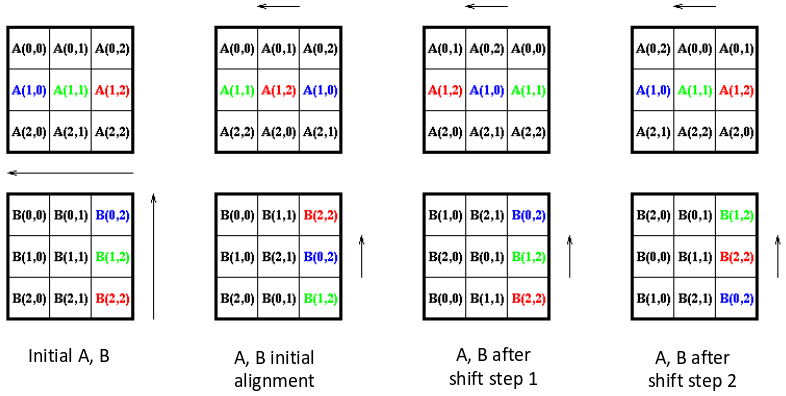
\includegraphics[width=.65\textwidth]{Pictures/Cannon.png}
\caption{Cannons's algorithm. Figure from \footfullcite{Xu2014}.}
\end{figure}
\end{center}
\begin{itemize}
\item good and simple on homogeneous 2D grid topology
\item provided implementation with blocking \lstinline{MPI_Send/MPI_Recv}
\item no initial alignment in provided implementation
\end{itemize}
\end{frame}

\subsection{Baseline}
\begin{frame}{\insertsubsection}
\begin{block}{Challenges:}
\begin{itemize}
	\item variance of test runs
	\item any more???
\end{itemize}
\end{block}

\begin{block}{Batch Script:}
\begin{itemize}
	\item writing output to file
		\lstinline[language=bash]{mpiexec -n 64 ./cannon$arch_ending $cannon_matrices_path/64x64-1.in $cannon_matrices_path/64x64-2.in | tee 64_$JOB_ID.out}
	\item postprocessing \lstinline{.out} files into \lstinline{.csv} files
	\item automation of job submission for multiple test runs	
\end{itemize}
\end{block}

\end{frame}

\subsection{Scaling}
\begin{frame}{\insertsubsection}
\begin{figure}
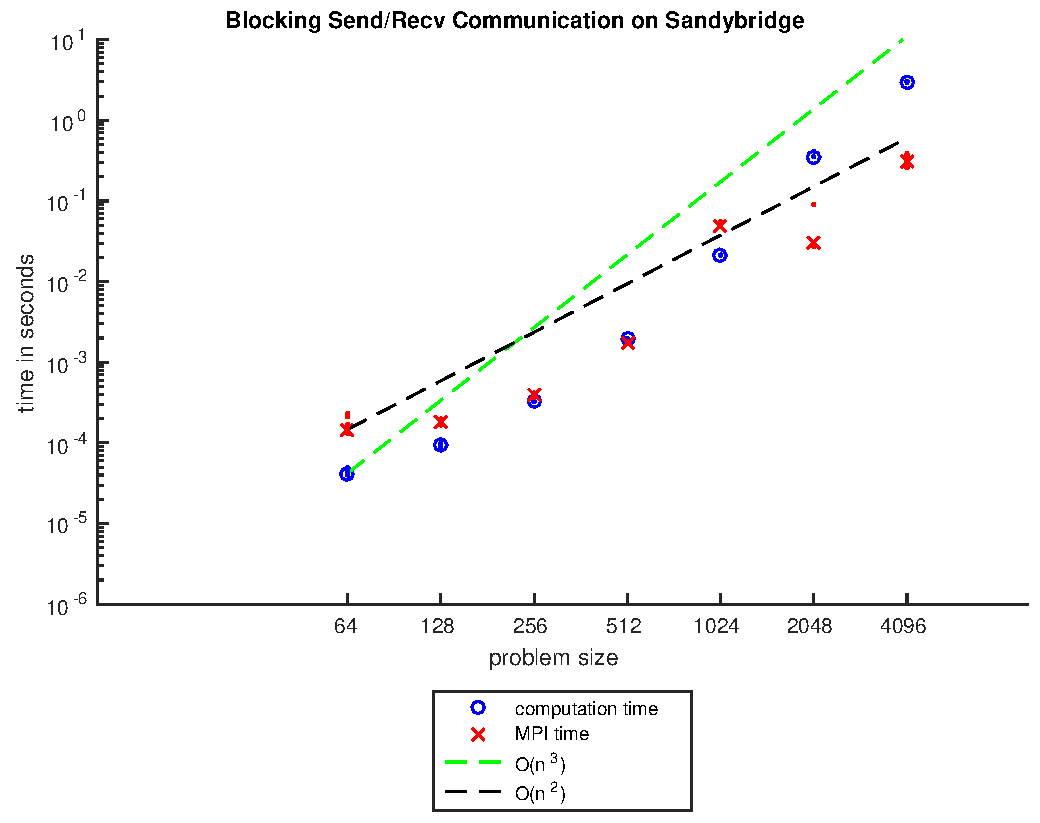
\includegraphics[width=.5\textwidth]{Pictures/Task3SB}
\hfill
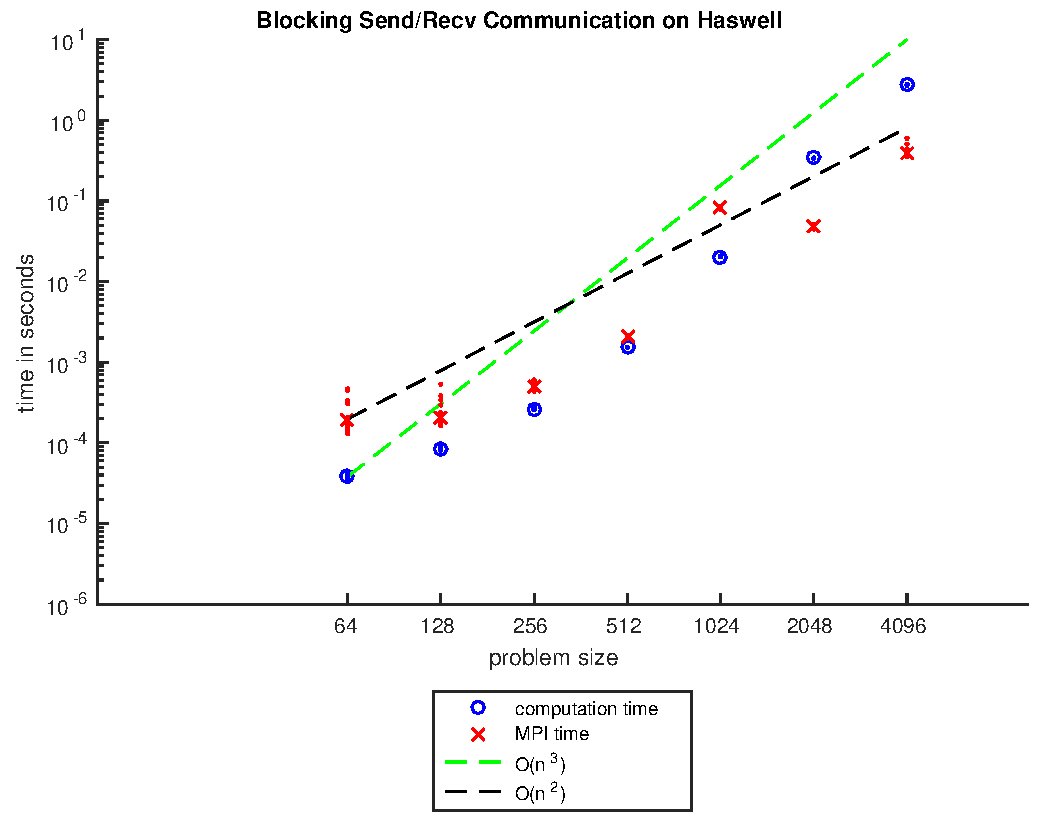
\includegraphics[width=.5\textwidth]{Pictures/Task3HW}
\end{figure}
\begin{itemize}
\item Communication and computation time match well with theoretical complexity.
\item Sandybride and Haswell similar, but Haswell has higher variance
\end{itemize}
\end{frame}

\section{MPI Point-to-Point Communication}
\begin{frame}{\phantom{Contents}}
\tableofcontents[
  currentsection  
]
\end{frame}
\subsection{MPI Non-Blocking Operations}
\begin{frame}{\insertsubsection}
\begin{itemize}
	\item Send/Receive
	\begin{itemize}
	\item \lstinline[basicstyle=\scriptsize\bf]{MPI_Isend}
	\item \lstinline[basicstyle=\scriptsize\bf]{MPI_Irecv}
	\end{itemize}

	\item Synchronization
	\begin{itemize}
	\item \lstinline[basicstyle=\scriptsize\bf]{MPI_Wait}
	\item \lstinline[basicstyle=\scriptsize\bf]{MPI_Probe}
	\end{itemize}
	
\end{itemize}
\end{frame}
\subsection{Optimizations}
\begin{frame}{\insertsubsection}
\begin{block}{What is overlap?}
We do not wait for either task to be completed, but try to do communication and computation at the same time. Therefore blocking communication cannot result in any overlap.
\end{block}
\begin{block}{What is the theoretical maximum overlap that can be achieved?}
Bounds for pure communication time: 
$$\max\left(0, T_\text{MPI}^\text{blocking} - T_\text{computation}\right) \leq T_\text{MPI}^\text{non-blocking} \leq T_\text{MPI}^\text{blocking}$$
As soon as $T_\text{computation}>T_\text{MPI}^\text{blocking}$, we can theoretically achieve 100\% overlap.
\end{block}
\begin{block}{Overheads}
\begin{itemize}
\item Copying into and from buffers
\item Initialization
\end{itemize}
\end{block}
\end{frame}

\begin{frame}[fragile]{\insertsubsection \ (contd.)}
\begin{block}{Was communication and computation overlap achieved?}
\begin{lstlisting}[language=C, basicstyle=\scriptsize, keepspaces=true, columns=flexible]
// cannon's algorithm
...
MPI_Request send_row_request;
MPI_Request send_column_request;
MPI_Request recv_row_request;
MPI_Request recv_column_request;
...
for(cannon_block_cycle = 0; cannon_block_cycle < sqrt_size; cannon_block_cycle++){
    ...
    // Horizontal communication
    MPI_Isend(...,row_communicator, &send_row_request);		
    MPI_Irecv(...,row_communicator, &recv_row_request);
    // Vertical communication
    MPI_Isend(...,column_communicator, &send_column_request);
    MPI_Irecv(...,column_communicator, &recv_column_request);
    ...		
    // computation heavy part 
    ...		
    MPI_Wait(&send_row_request, &status);
    MPI_Wait(&send_column_request, &status);
    MPI_Wait(&recv_row_request, &status);
    MPI_Wait(&recv_column_request, &status);
    ...		
}
\end{lstlisting}
\end{block}
\end{frame}

\subsection{Scaling}
\begin{frame}{\insertsubsection}
\begin{figure}
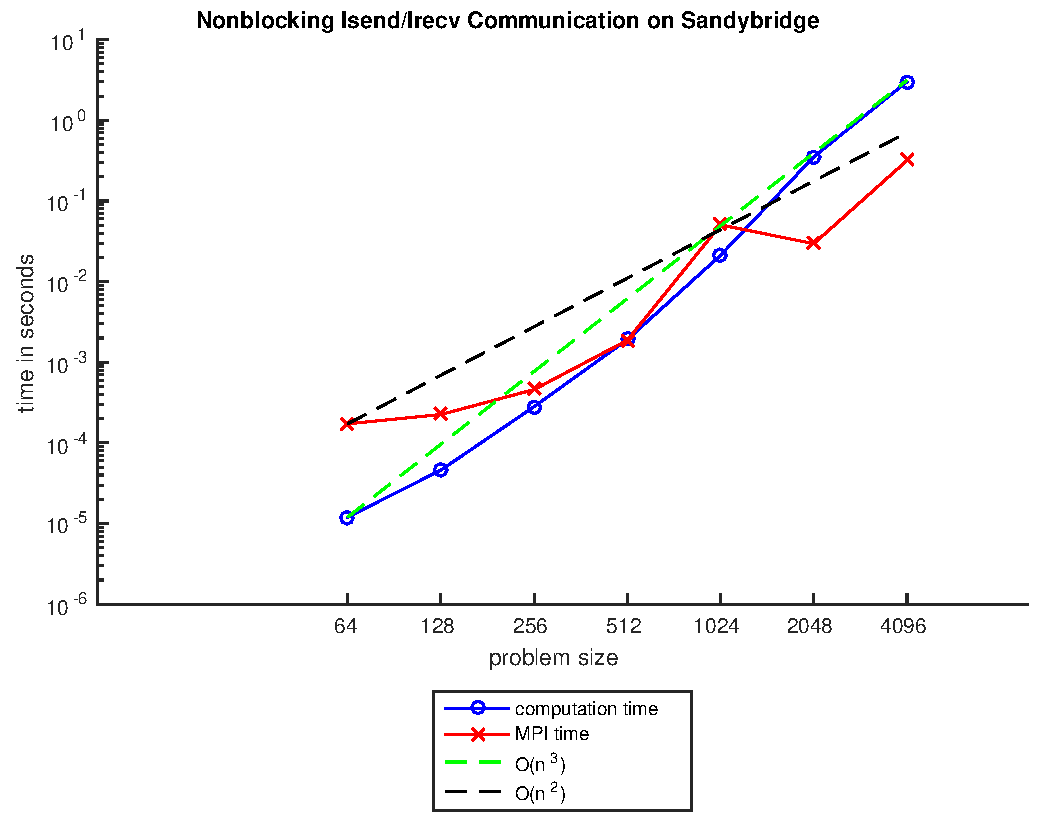
\includegraphics[width=.5\textwidth]{Pictures/Task4SB}
\hfill
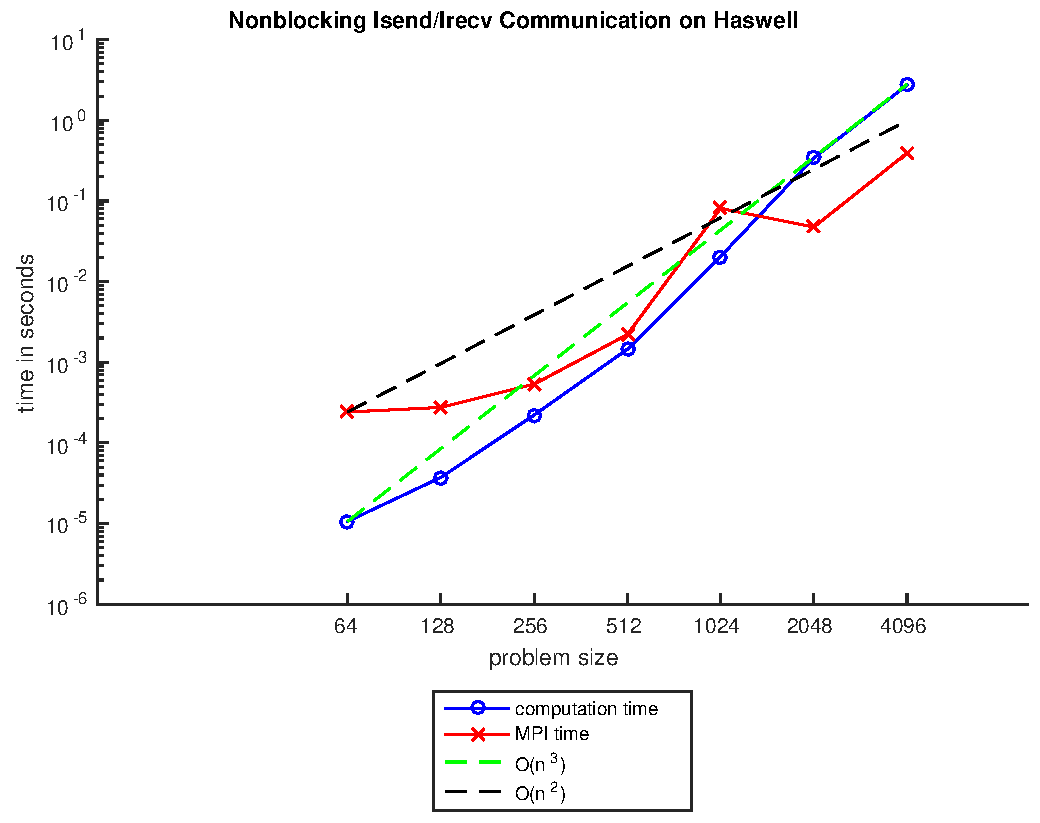
\includegraphics[width=.5\textwidth]{Pictures/Task4HW}
\end{figure}
\begin{itemize}
\item Only Little speedup.
\item No big differences between Haswell and Sandybridge.
\end{itemize}
\end{frame}

\begin{frame}{\insertsubsection \ (contd.)}
\begin{figure}
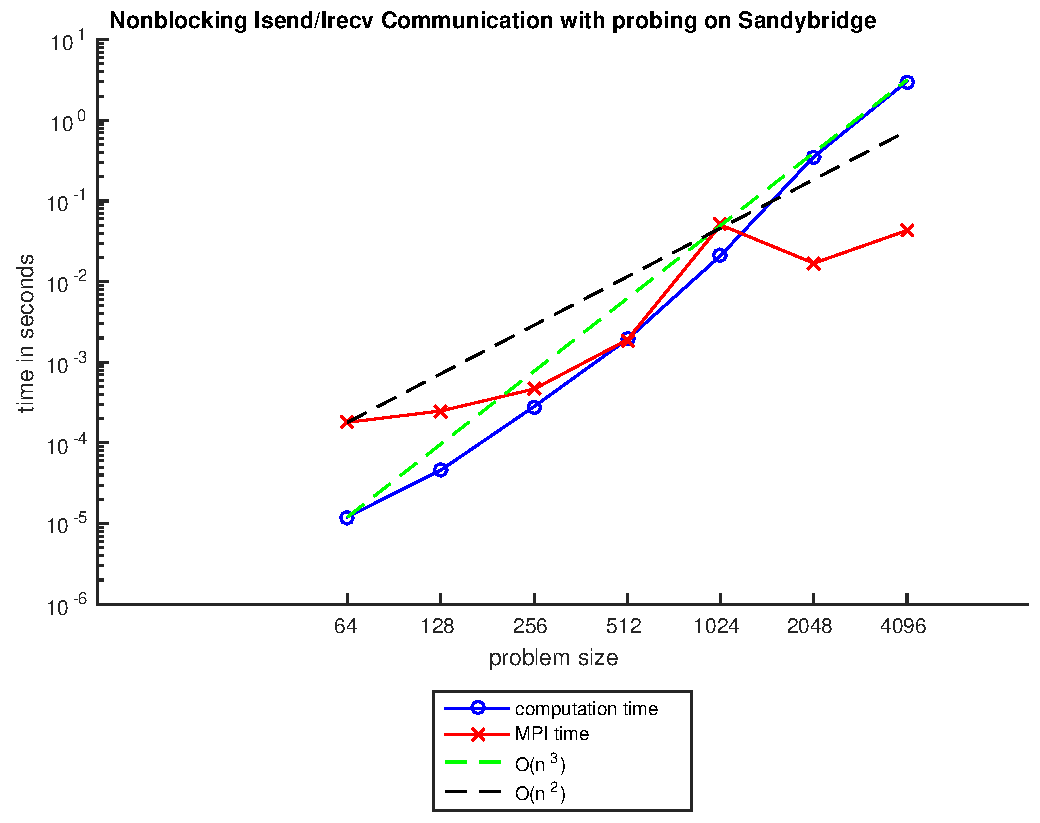
\includegraphics[width=.5\textwidth]{Pictures/Task4SBprobe}
\hfill
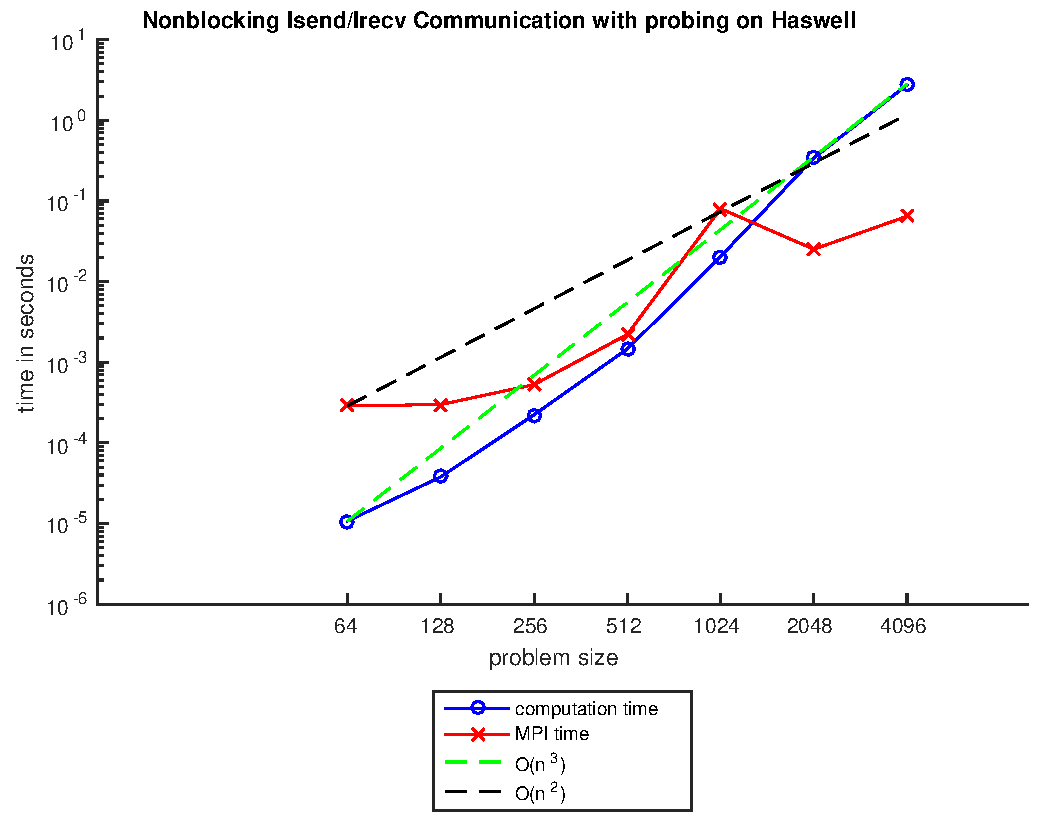
\includegraphics[width=.5\textwidth]{Pictures/Task4HWprobe}
\end{figure}
\begin{itemize}
\item using \lstinline{MPI_Probe}
\item big speedup
\item no big differences
\end{itemize}
\end{frame}

\section{MPI One-Sided Communication}
\begin{frame}{\phantom{Contents}}
\tableofcontents[
  currentsection  
]
\end{frame}
\subsection{MPI One-Sided Operations}
\begin{frame}{\insertsubsection}
\begin{itemize}
	\item Initialization
	\begin{itemize}
		\item \lstinline[basicstyle=\scriptsize\bf]{MPI_Win_create}
		\item \lstinline[basicstyle=\scriptsize\bf]{MPI_Win_free}
	\end{itemize}
	
	\item Remote Memory Access
	\begin{itemize}
		\item \lstinline[basicstyle=\scriptsize\bf]{MPI_Put}
		\item \lstinline[basicstyle=\scriptsize]{MPI_Get}
		\item \lstinline[basicstyle=\scriptsize]{MPI_Accumulate}                 
	\end{itemize}

	\item Synchronization
	\begin{itemize}
		\item \lstinline[basicstyle=\scriptsize\bf]{MPI_Win_fence}
		\item \lstinline[basicstyle=\scriptsize]{MPI_Win_post  /  MPI_Win_start /  MPI_Win_complete  / MPI_Win_wait}
		\item \lstinline[basicstyle=\scriptsize]{MPI_Win_lock / MPI_Win_unlock}
	\end{itemize}
\end{itemize}
\end{frame}


\subsection{Optimizations}
\begin{frame}[fragile]{\insertsubsection}
\begin{block}{Was communication and computation overlap achieved?}
\begin{lstlisting}[language=C, basicstyle=\scriptsize, keepspaces=true, columns=flexible]
// cannon's algorithm
...
MPI_Win_fence(0,win_A_even); 
...
for(cannon_block_cycle = 0; cannon_block_cycle < sqrt_size; cannon_block_cycle++){
    ...
    if(cannon_block_cycle%2==0){
        MPI_Win_fence(0,win_A_even);
        A_local_block = A_local_block_even;
        MPI_Win_fence(0,win_B_even);
        B_local_block = B_local_block_even;
        //Horizontal communication
        MPI_Put(..., win_A_odd);
        //Vertical communication
        MPI_Put(..., win_B_odd);
    }else{
        ... // odd and even are exchanged
    }
    ...
    // computation heavy part
}
\end{lstlisting}
\end{block}
\end{frame}

\subsection{Scaling}
\begin{frame}{\insertsubsection}
\begin{figure}
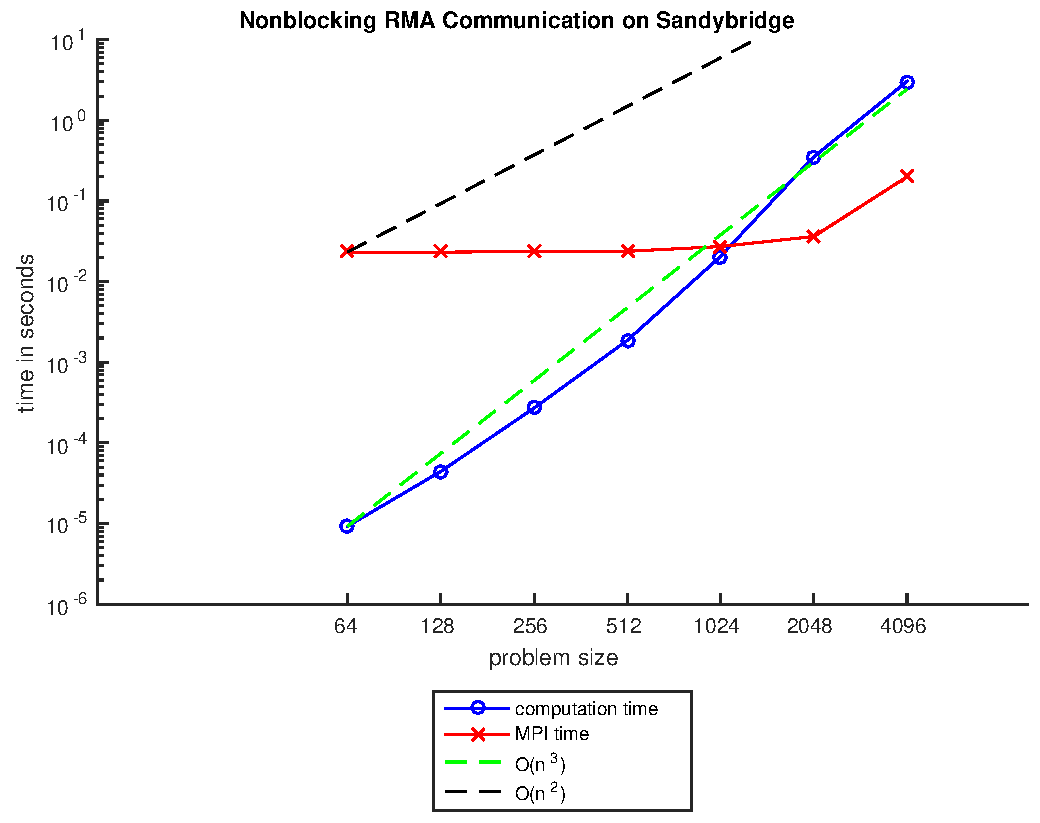
\includegraphics[width=.5\textwidth]{Pictures/Task5SB}
\hfill
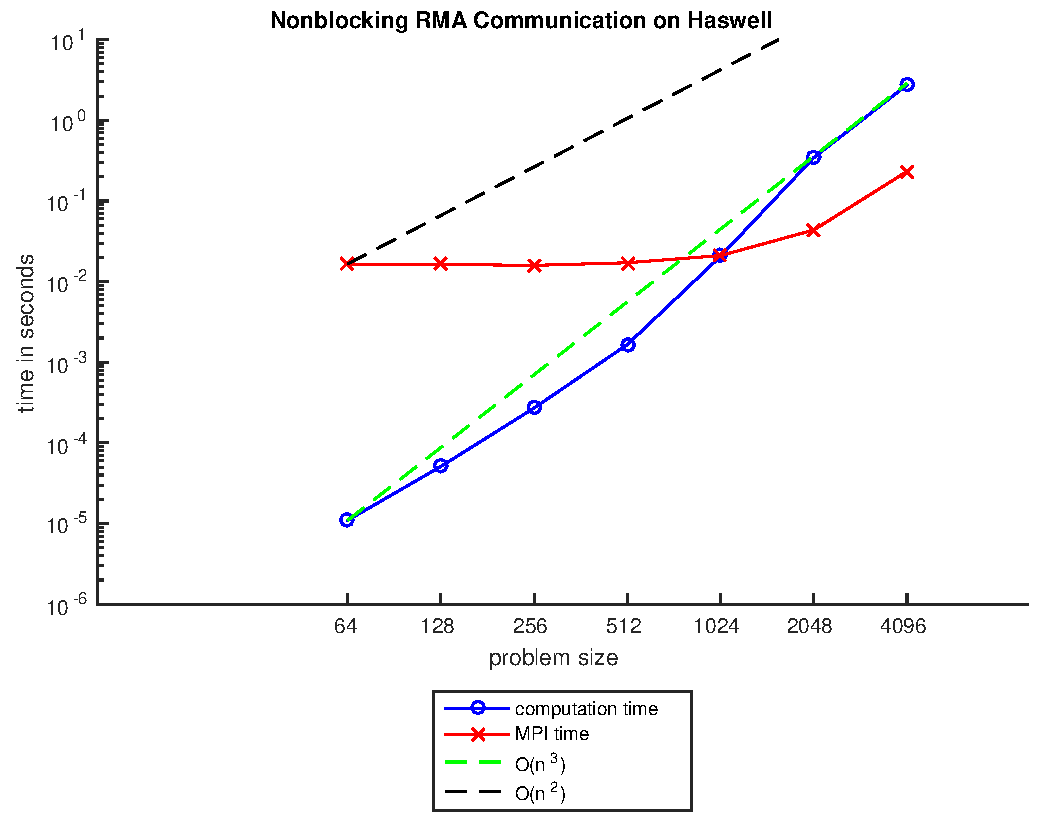
\includegraphics[width=.5\textwidth]{Pictures/Task5HW}
\end{figure}
\begin{itemize}
\item Good speedup for big size, very high overhead for small size.
\item No big differences between Haswell and Sandybridge.
\end{itemize}
\end{frame}

\section{Overall Comparison}
\begin{frame}{\phantom{Contents}}
\tableofcontents[
  currentsection  
]
\end{frame}

\begin{frame}{Speedup of communication time}
\begin{figure}
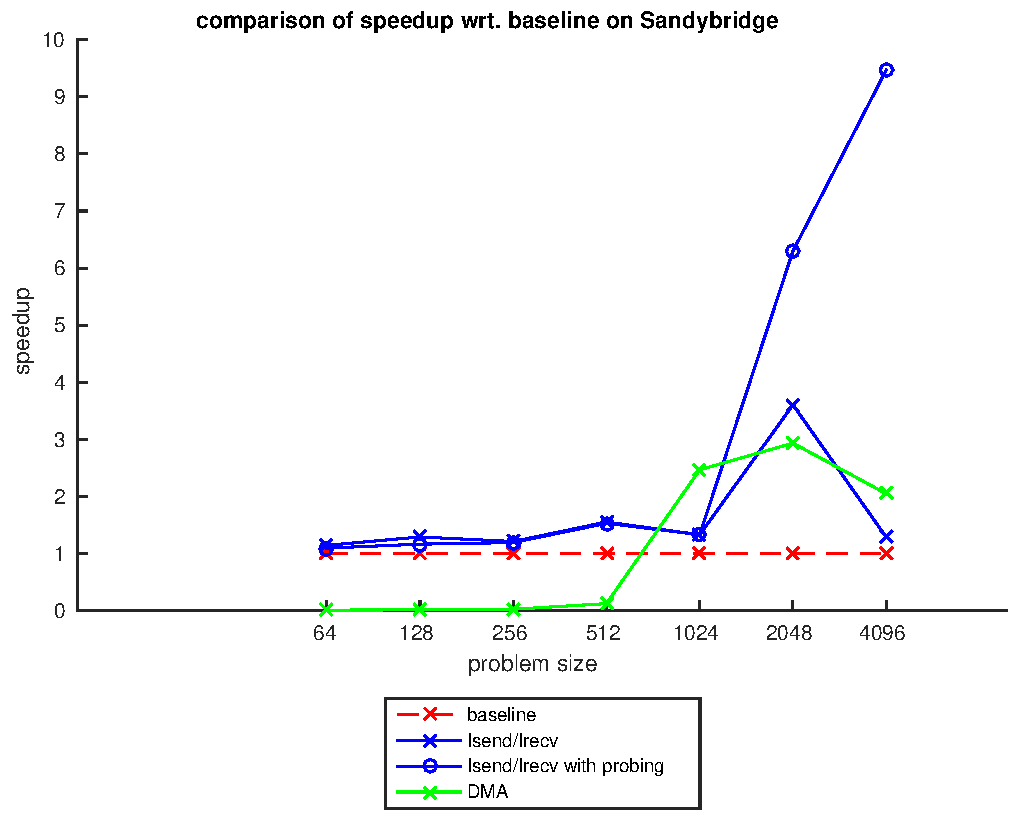
\includegraphics[width=.5\textwidth]{Pictures/comparisonSB}
\hfill
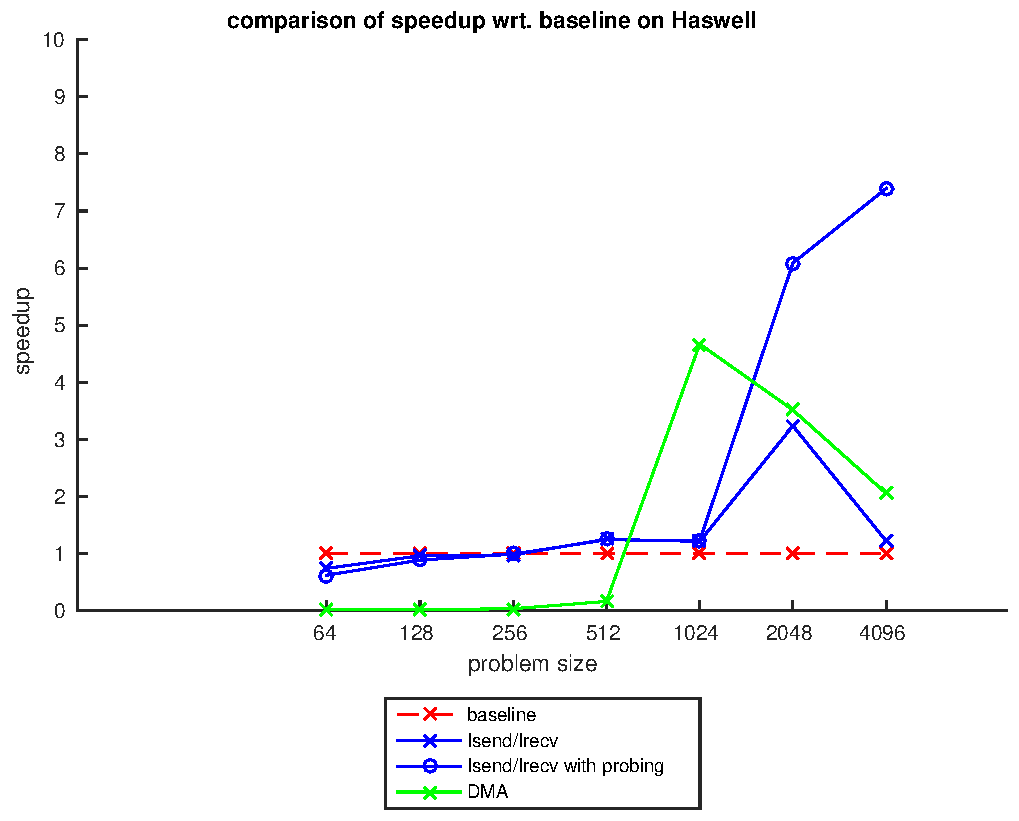
\includegraphics[width=.5\textwidth]{Pictures/comparisonHW}
\end{figure}
\begin{itemize}
\item \textbf{Nonblocking:} Usually little speedup, but big speedup for $2048\times2048$.
\item \textbf{Nonblocking with probing:} High speedup for big problems.
\item \textbf{DMA:} High overhead, but good speedup for big problems.
\end{itemize}

\end{frame}


\end{document}
